\documentclass[11pt,a4paper]{article}

% Packages
\usepackage[utf8]{inputenc}
\usepackage[T1]{fontenc}
\usepackage{CJKutf8}
\usepackage[margin=1in]{geometry}
\usepackage{amsmath,amssymb,amsthm}
\usepackage{graphicx}
\usepackage{subcaption}
\usepackage{hyperref}
\usepackage{listings}
\usepackage{xcolor}
\usepackage{booktabs}
\usepackage{enumitem}
\usepackage{fancyhdr}

% Code listing style
\lstset{
    basicstyle=\ttfamily\small,
    breaklines=true,
    frame=single,
    numbers=left,
    numberstyle=\tiny\color{gray},
    keywordstyle=\color{blue},
    commentstyle=\color{green!60!black},
    stringstyle=\color{red},
    showstringspaces=false,
    tabsize=4
}

% Header and footer
\pagestyle{fancy}
\fancyhf{}
\lhead{COMP4901B - Large Language Models}
\rhead{Assignment 1}
\cfoot{\thepage}
\setlength{\parindent}{0pt}

% Title information
\title{
    \textbf{COMP4901B: Large Language Models} \\
    \vspace{0.5em}
    \Large Assignment 1 Report
}
\author{HE, Wenqian \\ Student ID: 20860896}
\date{\today}

\begin{document}

\maketitle


\section{Part 1: Data Preprocessing}

\subsection{Cleaning Logic}

For each paragraph in the text, I do the following cleaning steps:
\begin{itemize}
    \item if there are at least 101 consecutive alphanumeric characters, I remove the paragraph
    \item if the paragraph has no punctuation, I remove the paragraph
\end{itemize}

\subsection{Heuristic Quality Filter Logic}

I reject the text if:

\begin{itemize}
    \item there are any bad words in the text
    \item the text has no punctuation
    \item the text has no non-whitespace or punctuation characters
    \item the ratio of alphanumeric, punctuation, or whitespace characters to the total number of characters is less than 0.8
\end{itemize}

\subsection{English Text Detection Logic}

First, I filter the alphabetic characters, such as "a", "B", "\begin{CJK}{UTF8}{gbsn}我\end{CJK}", etc., excluding the symbols like "?", "/", "-", etc.

Then, from the remaining alphabetic characters, I count the number of English alphabetic characters (i.e. "a-zA-Z").

If the ratio of English alphabetic characters to the total number of alphabetic characters is greater than the English character ratio threshold (I use 0.99 as the threshold), I accept the text.

\subsection{Results}

Here is the record numbers of WARC records processed and the number that pass all filters:


\begin{lstlisting}
python homework.py --fname data.warc --output cleaned_test.txt --dfname topic_dataset.json --num_records 2000

704 passed out of 2000 records processed.
Cleaned documents saved to: cleaned_test.txt
121 deduplicated out of 219 records processed.
\end{lstlisting}

\section{Part 2: Pretraining}

The model is trained on Mac book with mps device enabled, which is achieved by modifying the \texttt{run\_llama.py} file. This training takes about 9 hours.

Here is the training command:
\begin{lstlisting}
python run_llama.py \
  --run_name run7 \
  --option pretrain \
  --data_path train_100M \
  --block_size  256 \
  --batch_size 512 \
  --micro_batch_size 32 \
  --epochs 1 \
  --tokenized_dir train_100M/tokenized \
  --use_gpu  \
  --val_path dev \
  --val_tokenized_dir dev/tokenized \
  --val_per_steps 200 \
  --test_path  test \
  --test_tokenized_dir test/tokenized \
  --auto_resume \
  --warmup_ratio 0.1 \
  --lr 1e-3 
\end{lstlisting}

The training loss declines quickly at the beginning, and then keep declining stably.

Here are some important curves:

\begin{figure}[h!]
    \centering
    \begin{subfigure}[b]{0.48\textwidth}
        \centering
        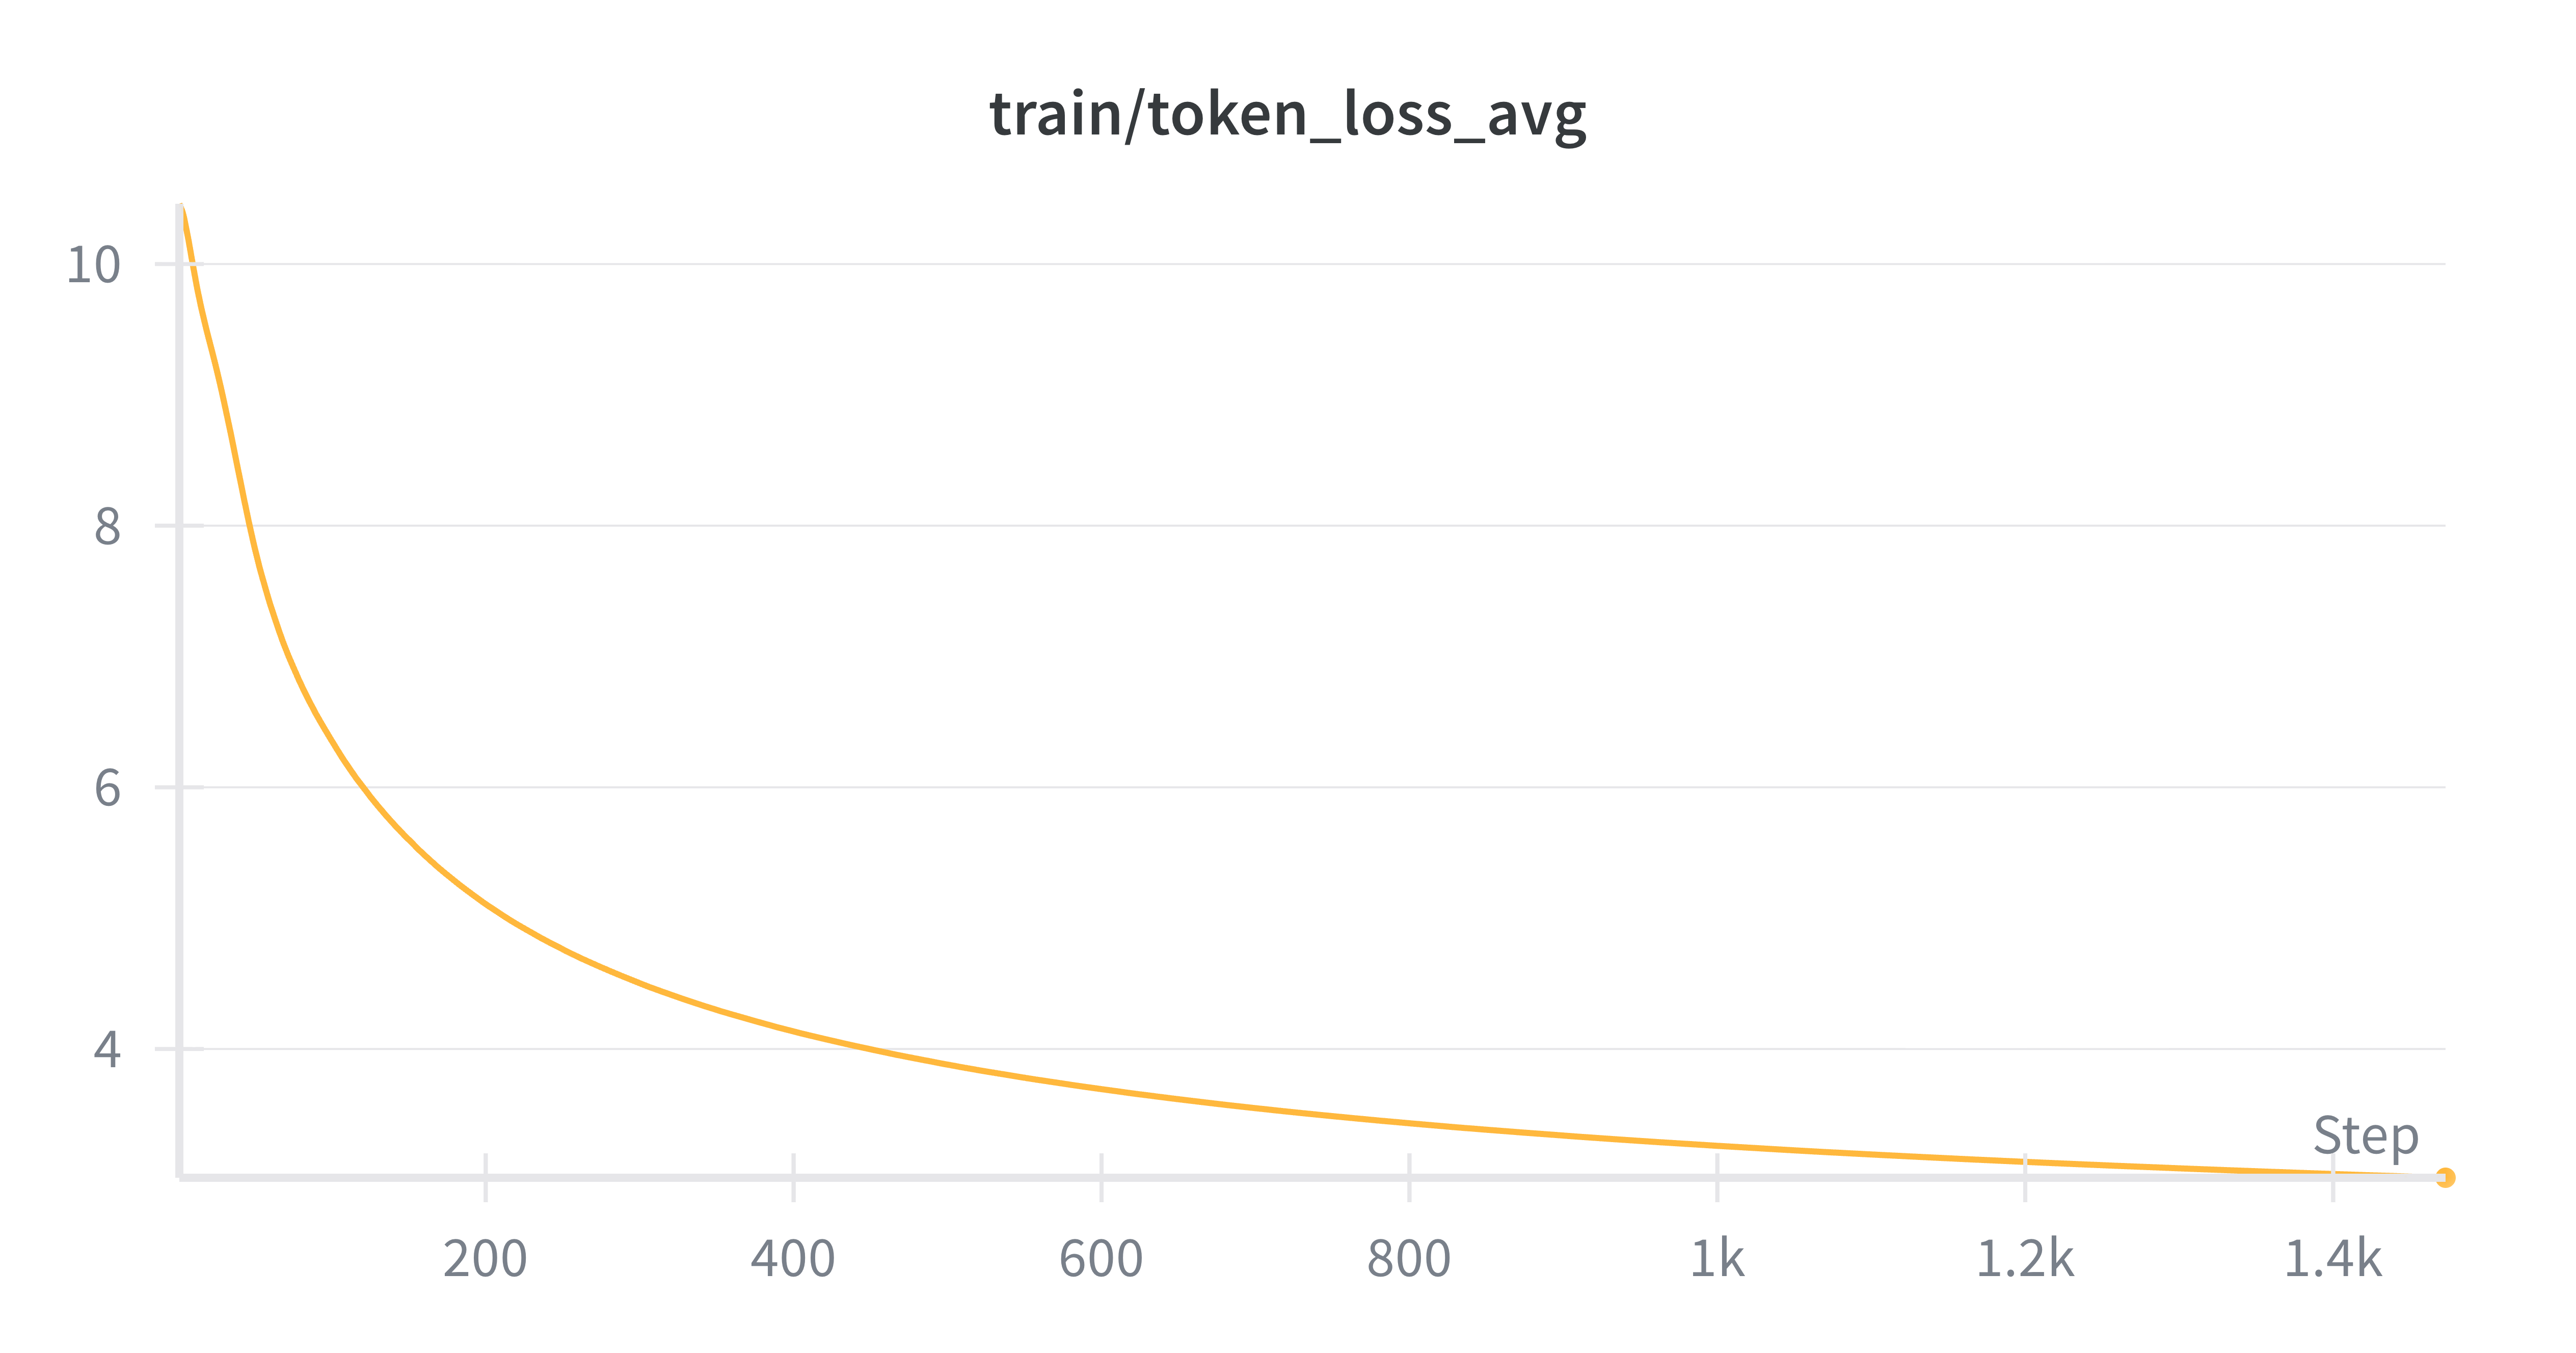
\includegraphics[width=\textwidth]{train_loss_avg.png}
        \label{fig:train_loss}
    \end{subfigure}
    \hfill
    \begin{subfigure}[b]{0.48\textwidth}
        \centering
        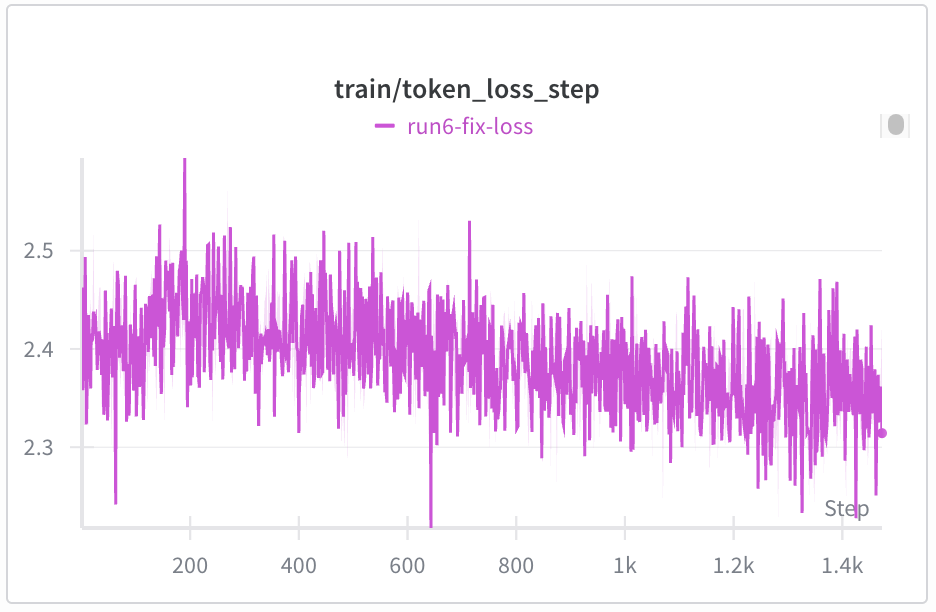
\includegraphics[width=\textwidth]{train_loss_step.png}
        \label{fig:train_loss_step}
    \end{subfigure}
    
    \vspace{0.5em}
    
    \begin{subfigure}[b]{0.48\textwidth}
        \centering
        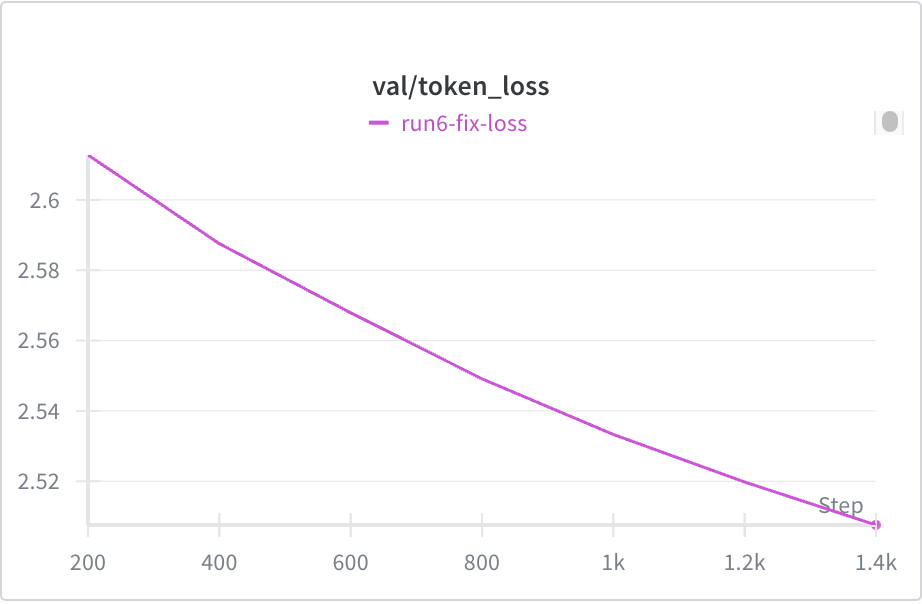
\includegraphics[width=\textwidth]{val_loss.png}
        \label{fig:val_loss}
    \end{subfigure}
    \hfill
    \begin{subfigure}[b]{0.48\textwidth}
        \centering
        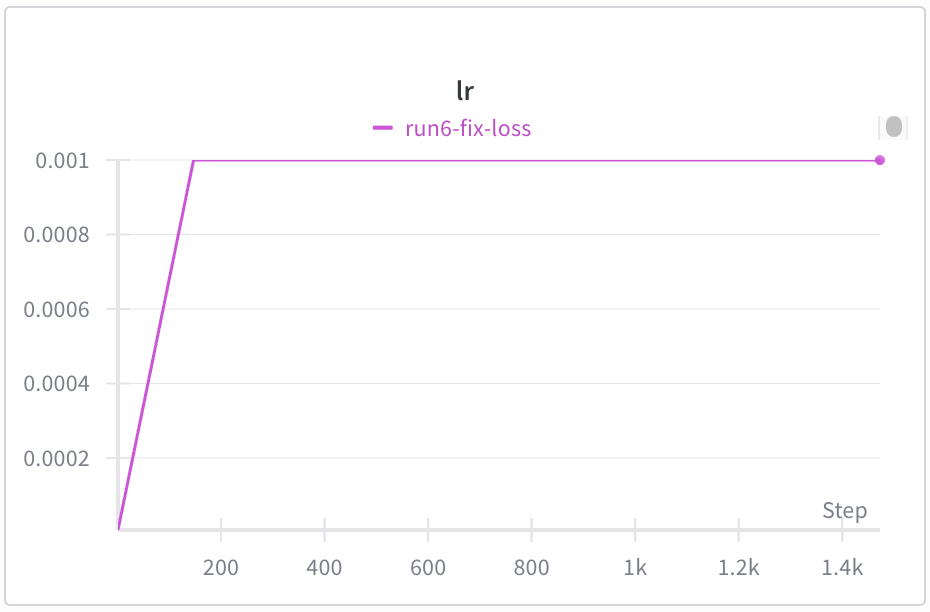
\includegraphics[width=\textwidth]{lr.png}
        \label{fig:lr}
    \end{subfigure}
    
    \caption{Training metrics visualization}
    \label{fig:training_metrics}
\end{figure}

\section{Part 3: Generation}


Provided model:

\begin{lstlisting}
python run_llama.py --pretrained-model-path llama2-42M-babylm.pt --option generate

// temperature = 0.0
White Bird is a 2023 American war drama movie starring Diana Hunt, Diana Hunt, Diana Hunt, Diana Hunt, Diana Hunt, Diana Hunt, Diana Hunt, Diana Hunt, Diana Hunt, Diana Hunt, Diana Hunt, Diana Hunt, Diana Hunt, Diana Hunt, Diana Hunt,

// temperature = 0.5
White Bird is a 2023 American war drama movie starring James Dee, Eddie Quinn, Larry Dee, James McDonald, George J. L. Smith, David Dee, John Duck, James McDonald, John H. W. Bush. It was distributed by 20th Century Fox. = = = PG4021 = = = A LITTLE
\end{lstlisting}


My pretrained model:
\begin{lstlisting}
python run_llama.py --pretrained-model-path run7-pretrain-1-0.001.pt --option generate

// temperature = 0.0
White Bird is a 2023 American war drama movie starring John H. W. Bush, John H. W. Bush, John H. W. Bush, John H. W. Bush, John H. W. Bush, John H. W. Bush, John H. W. Bush, John H. W. Bush, John H. W. Bush, John H. W. Bush, John H. W.

// temperature = 0.5
White Bird is a 2023 American war drama movie starring Shon Alley and Kyle, Marvin, John H. Sharine, Danny Reed, David H. W. Bush, J. W. Bush, David H. W. Bush, David H. Bush, Daniel H. Bush, David H. W. Bush, Michael Jackson, David K. Bush, David H. Bush, James K
\end{lstlisting}


From the generation results, although using temperature = 0.0 is more coherent, such as the generated sentence from my pretrained model, which echos "John H. W. Bush" again and again, I think the temperature = 0.5 is better. Using greedy method will lead to very repetitive and boring generation, as shown in the generated sentence from the both models. Using temperature sampling will lead to more diverse and interesting generation.


\end{document}

